\documentclass[11pt]{article}

\usepackage[margin=2cm]{geometry}
\usepackage{titling}
\usepackage[T1]{fontenc}
\usepackage{tabularx}
\usepackage{amsfonts}
\usepackage{amsmath}
\usepackage{mathdots}
\usepackage{stackengine}
\usepackage{graphicx}
\usepackage{subcaption}
\usepackage{changepage}
\usepackage{algorithm}
\usepackage[noend]{algpseudocode}

\usepackage{listings}
\lstdefinelanguage{Julia}
  {
    morekeywords={struct,function,if,for,end},
    sensitive=true,
    alsoother={\$},
    morecomment=[l]\#,
    morestring=[b]",
  }[keywords]
\lstset{
    language=Julia,
    basicstyle=\small\ttfamily,
    keywordstyle=\bfseries,
    showstringspaces=false,
    breaklines=true,
    captionpos=b,
}

\pretitle{\begin{center}\Huge\bfseries}
\posttitle{\par\end{center}\vskip 0.5em}
\preauthor{\begin{center}\Large}
\postauthor{\end{center}}
\predate{\par\large\centering}
\postdate{\par}

\title{Obliczenia naukowe - lab 5}
\author{Jakub Musiał 268442}
\date{Styczeń 2024}

\begin{document}

\maketitle

\hspace{1cm}

\noindent\textbf{Oznaczenie: } $n \in \mathbb{N} \implies [n] = \{1, ..., n\}$

\section*{Opis problemu}
    Zadaniem jest przygotowanie biblioteki (modułu w języku \texttt{Julia}) o nazwie \texttt{blocksys},
    która umożliwi efektywne rozwiązywanie układów równań liniowych reprezentowanych macierzowo:
    $$ Ax = b $$
    Gdzie $A \in \mathbb{R}^{n \times n}$ - macierz współczynników, $b \in \mathbb{R}^n$ - wektor prawych stron oraz
    $x \in \mathbb{R}^n$ - szukane rozwiązanie.
    \newline\newline
    Dodatkowo wiemy, że $A$ jest macierzą blokową o następującej strukturze:
    $$
    A =
    \begin{bmatrix}
    A_1    & C_1    & 0      & 0       & 0         & \dotsb  & 0       \\
    B_2    & A_2    & C_2    & 0       & 0         & \dotsb  & 0       \\
    0      & B_3    & A_3    & C_3     & 0         & \dotsb  & 0       \\
    \vdots & \ddots & \ddots & \ddots  & \ddots    & \ddots  & \vdots  \\
    0      & \dotsb & 0      & B_{v-2} & A_{v-2}   & C_{v-2} & 0       \\
    0      & \dotsb & 0      & 0       & B_{v-1}   & A_{v-1} & C_{v-1} \\
    0      & \dotsb & 0      & 0       & 0         & B_{v}   & A_{v}
    \end{bmatrix}
    $$
    Gdzie:
    \begin{itemize}
        \item $0 \in \mathbb{R}^{l \times l}$ - kwadratowa macierz zerowa
        \item $v = \frac{n}{l}$ - wymiar macierzy blokowej A dla bloków wymiaru $l \times l$ (zakładając, że $l | n$)
        \item $k \in [v] \implies A_k \in \mathbb{R}^{l \times l}$ - kwadratowa macierz gęsta
        \item
            $
            k \in \{2, ..., v\} \implies B_k \in \mathbb{R}^{l \times l}
            \land B_k =
            \begin{bmatrix}
                0      & \dotsb & 0      & b^k_1  \\
                0      & \dotsb & 0      & b^l_2  \\
                \vdots & \ddots & \vdots & \vdots \\
                0      & \dotsb & 0      & b^k_l
            \end{bmatrix}
            $
        \item
            $
            k \in [v - 1] \implies C_k \in \mathbb{R}^{l \times l}
            \land C_k =
            \begin{bmatrix}
                c^k_1  & 0      & 0      & \dotsb    & 0      \\
                0      & c^k_2  & 0      & \dotsb    & 0      \\
                \vdots & \ddots & \ddots & \ddots    & \vdots \\
                0      & \dotsb & 0      & c^k_{l-1} & 0      \\
                0      & \dotsb & 0      & 0         & c^k_l
            \end{bmatrix}
            $
    \end{itemize}

    \newpage

    \noindent
    Znając strukturę macierzy $A$ można zdefiniować efektywne pamięciowo struktury przechowujące taką macierz. Taką strukturę można zdefiniować na wiele sposobów, jednak w swoich eksperymentach korzystałem z dwóch implementacji:
    \newline

    \subsubsection*{Implementacja ogólna:}
        \begin{lstlisting}
            struct DictMatrix
                n::Int64
                l::Int64
                M::Dict{Tuple{Int64, Int64, Float64}}
            end
        \end{lstlisting}

        \noindent
        Elementy niezerowe macierzy są przechowywane w słowniku, gdzie kluczem jest para indeksów $(i, j)$ takich, że $i$ - indeks wiersza oraz $j$ - indeks kolumny.
        \newline
        Pobranie elementu z indeksu $(i, j)$ zwraca wartość z tego indeksu, jeśli jest on kluczem w słowniku albo $0$ w przeciwnym przypadku.
        \newline
        Przypisanie wartości elementowi na indeksie $(i, j)$ przypisuje zadaną wartość do klucza $(i, j)$ w słowniku, jeśli wartość ta nie jest zerem. W przeciwnym przypadku klucz $(i, j)$ jest usuwany ze słownika.
        \newline\newline
        Tak zdefiniowana struktura przechowuje wyłącznie niezerowe elementy, zatem na podstawie struktury macierzy A możemy zauważyć (wiedząc, że $l$ jest stałe), że złożoność pamięciowa takiej struktury jest liniowa:
        $$ M_A : O(v \cdot l^2) = O(\frac{n}{l} \cdot l^2) = O(n \cdot l) = O(n) $$
        $$ M_B = M_C : O((v - 1) \cdot l) = O((\frac{n}{l} - 1) \cdot l) = O(n - l) = O(n) $$
        \noindent
        Dodatkowo możemy zauważyć, ze koszt zamortyzowany operacji pobrania oraz ustawienia elementu ze słownika jest stały ($O(1)$), jednak przy bardzo dużych macierzach istnieje ryzyko występowania kolizji funkcji hashującej, co może pogorszyć złożoność czasową tych operacji. Niestety jest to nieuniknione dla tak zdefiniowanej struktury ogólnej, która nie zakłada nic o postaci przechowywanej macierzy.
        \newline

    \subsubsection*{Implementacja uwzględniająca postać macierzy $A$:}
        \begin{lstlisting}
            struct Matrix
                n::Int64
                l::Int64
                A::Vector{Matrix{fl}}
                B::Vector{Vector{fl}}
                C::Vector{Matrix{fl}}
            end

            function QCMatrix(n::int, l::int)
                v = div(n, l)
                A = [zeros(fl, l, l) for _ in 1:v]
                B = [zeros(fl, l) for _ in 2:v]
                C = [zeros(fl, l, l) for _ in 1:v-1]
                new(n, l, A, B, C)
            end
        \end{lstlisting}

        \noindent
        Znając specyficzną strukturę macierzy $A$ możemy zaimplementować bardziej dokładną strukturę opisującą taką macierz. Musimy zatem przechowtywać wyłącznie bloki $A_k : k \in [v]$, $B_k : k \in \{2, ..., v\}$ oraz $C_k : k \in [v - 1]$. Przeprowadziwszy rozumowanie analogiczne do tego dla struktury ogólnej, możemy zauważyć, że złożoność pamięciowa jest liniowa dla stałego $l$ (przechowanie bloków $C_k$ jako macierze jest konieczne ze względu na operacje wykonywane na macierzy w zadanych algorytmach).
        $$ M_A : O(v \cdot l^2) = O(\frac{n}{l} \cdot l^2) = O(n \cdot l) = O(n) $$
        $$ M_B : O((v - 1) \cdot l) = O((\frac{n}{l} - 1) \cdot l) = O(n - l) = O(n) $$
        $$ M_C : O((v - 1) \cdot l^2) = O((\frac{n}{l} - 1) \cdot l^2) = O(nl - l^2) = O(n) $$
        \noindent
        Dla tak zdefiniowanej struktury operacja pobrania wartości z $i$-tej kolumny i $j$-tego rzędu polega na sprawdzeniu, do którego bloku należy podana para indeksów i zwrócenie wartości z odpowiedniego bloku lub zera, jeśli $(i, j)$ nie znajduje się w żadnym z bloków. Analogicznie przypisanie wartości zmienia element w macierzy wyłącznie jeśli $(i, j)$ jest w jednym z przechowywanych bloków.
        \newline
        Przynależność pary indeksów $(i, j)$ do poszczególnych bloków możemy zdefiniować następująco:
        \newline\newline
        Niech: $ r_b = \lfloor \frac{i - 1}{l} \rfloor + 1 \land c_b = \lfloor \frac{j - 1}{l} \rfloor + 1 $
        \newline
        Wtedy:
        $$ c_b = r_b \implies "(i, j) \in A_{r_b}" $$
        $$ c_b = r_b - 1 \implies "(i, j) \in B_{r_b - 1}" $$
        $$ c_b = r_b + 1 \implies "(i, j) \in C_{r_b}" $$
        \newline
        Możemy zauważyć, że takie operacje na macierzy wykonują się zawsze w czasie stałym, zatem możemy się spodziewać, że dla dużych macierzy wejściowych, algorytmy implementowane algorytmy będą się wykonywały szybciej niż dla struktóry ogólnej - \texttt{DictMatrix}.

    \newpage

\section*{Zadanie 1}
    \subsection*{Problem}
        Zaimplementować funkcję rozwiązującą układ równań liniowych zadanych przez wyrażenie macierzowe
        $$ Ax = b $$
        za pomocą eliminacji Gaussa oraz eliminacji Gaussa z częściowym wyborem elementu głównego, uwzględniając specyficzną strukturę macierzy $A$.

    \subsection*{Rozwiązanie}
        Metoda eliminacji Gaussa polega na zerowaniu elementów pod przekątną macierzy, iterując po jej kolumnach tak, że w rezultacie otrzymujemy macierz górno trójkątną.

        \begin{algorithm}[h!]
        \caption{Eliminacja Gaussa}
        \label{alg:gauss_elimination_default}
        \begin{algorithmic}[1]
            \Require $A, b, n, l$
            \For{$k \gets 1$ to $n - 1$}
                \For{$i \gets k + 1$ to $n$}
                    \State $l_{ik} \gets \frac{A_{ik}}{A_{kk}}$
                    \For{$j \gets k + 1$ to $n$}
                        \State $A_{ij} \gets A_{ij} - l_{ik} \cdot A_{kj}$
                    \EndFor
                    \State $b_i \gets b_i - l_{ik} \cdot b_k$
                \EndFor
            \EndFor
            \State \Return $(A, b)$
        \end{algorithmic}
        \end{algorithm}

        \noindent
        Widzimy jednak, że ten algorytm ma złożoność obliczeniową $O(n^3)$, co wynika z trzech zagnieżdżonych pętli, których liczba iteracji jest zależna od rozmiaru macierzy $A$. Wiemy jednak, że pod przekątną zadanej macierzy jest wiele zer, co pozwoli nam przyspieszyć opisany powyżej algorytm. Aby to zrobić będziemy chcieli w wewnętrznych pętlach iterować od przekątnej do ostatniego niezerowego elementu.
        \newline\newline
        Rozważmy zatem pętlę z linii $2$, w której iterujemy po rzędach od $(k + 1)$-ego do ostatniego.
        Wiemy jednak, że pod przekątną w $k$-tej kolumnie jest dokładnie $\min\{l - (k \mod l), n - k\}$ (zakładając, że indeksujemy od $1$). Wynika to z faktu, że przechodząc po przekątnej zawsze jesteśmy w bloku $A_i$, zatem musimy wyzerować elementy pod przekątną w podmacierzy $A_i$ oraz wszystkie elementy z podmacierzy $B_{i + 1}$ - dokładnie $l$ elementów w kolumnie $k = i \cdot l$, dla której $l - (i \cdot l \mod l) = l - 0 = l$. Musimy jednak uwzględnić także ostatnie bloki w macierzy, dla których $l - (k \mod l) > n$. Stąd możemy zamienić ogranicznie $i \in \{k + 1, ..., n\}$ w pętli z linii $2$ na $i \in \{k + 1, min\{k + l - (k \mod l), n\}\}$.
        \newline\newline
        Analogiczne rozumowanie możemy przeprowadzić dla pętli z linii $4$. Tutaj wiemy, że dla każdego $k$ będziemy modyfikowali wartości wyłącznie pomiędzy przekątnymi podmacierzy $A_i$ oraz przekątnymi podmacierzy $C_i$. Zauważmy, że te przekątne są do siebie "równoległe" oraz w odległości $l$. Zatem wystarczy, że będziemy rozpatrywać tylko $l$ elementów na prawo od przekątnej, jednak musimy ponownie uwzględnić ostatnie bloki macierzy. Stąd możemy zamienić ogranicznie pętli z linii $4$ z obecnego $j \in \{k + 1, ..., n\}$ na $j \in \{min\{k + l, n\}\}$.
        \newline\newline
        Taka modyfikacja algorytmy eliminacji Gaussa gwarantuje nam złożoność liniową: najbardziej zewnętrzna pętla wykonuje się $n$ razy, a pętle wewnętrzne $O(l)$ razy. Zatem, wiedząc, że $l$ jest stałą, całkowita złożoność obliczeniowa zmodyfikowanego algorytmu to $O(n * l^2) = O(n)$.

        \newpage

        \noindent
        Algorytm eliminacji Gaussa z wyborem elementu głównego różni się od standardowego algorytmu tym, że dla każdej kolumny przed wykonaniem kroku eliminacji szukamy elementu o maksymalnej wartości bezwzględnej oraz zamieniami miejscami rząd obecny z tym, w którym znajduje się znaleziony element (o ile element maksymalny nie znajduje się w aktualnym rzędzie).
        \newline
        Zabieg ten ma na celu zminimalizowanie błędów oblczeniowych wynikających z występowania wartości $\varepsilon \approx 0$ na przekątnej badanej macierzy. Dla takiej sytuacji w $k$-tym kroku eliminacji gaussa otrzymujemy:
        $$ l_{ik} = \frac{A_{ik}}{A_{kk}} = \frac{A_{ik}}{\varepsilon} = A_{ik} \cdot \varepsilon^{-1} $$
        \noindent
        \newline
        Zauważmy, że dla małych wartości $\varepsilon$ ($< \epsilon_{mach}$) powyższe wyrażenie oraz późniejsze obliczenia mogą być numerycznie niepoprawne ze względu na ograniczoną precyzję arytmetyki.
        \newline\newline
        Zatem wybór elementu głównego powinien zapobiec błędom obliczeniowym wynikającym z występowania wartości bliskich zeru na przekątnej macierzy.
        \newline
        Dodatkowo możemy zauważyć, że struktura macierzy $A$ pozwala nam na zawężenie obszaru poszukiwań takiego elementu - ostatnim rzędem zawierającym element niezerowy w $k$-tej kolumnie będzie rząd $r_{max} =  min\{k + l - (k \mod l), n\}$ (jak w poprzednim algorytmie). W związku z zamianą rzędów macierzy musimy również rozważyć maksymalny zakres kolumn w najbardziej wewnętrznej pętli - tutaj nie mamy stałej odległości między przekątną, a elementem z bloku $C_k$, zatem musimy uwzględnić wszystkie kolumny z bloku $C_k$. Stąd otrzymujemy zmodyfikowany algorytm eliminacji Gaussa z częściowym wyborem elementu głównego:

        \begin{algorithm}[h!]
        \caption{Eliminacja Gaussa z częściowym wyborem elementu głównego}
        \label{alg:gauss_elimination_partial_pivot}
        \begin{algorithmic}[1]
            \Require $A, b, n, l$
            \For{$k \gets 1$ to $n - 1$}
                \State $r_{max} \gets min\{k + l - (k \mod l), n\}$
                \State $r_{v_{max}} \gets k + argmax_{i \in \{k, ..., r_{max}\}}(|A_{i, k}|) - 1$

                \If{$r_{v_{max}} \ne k$}
                    \State $swap\_rows(A, k, r_{v_{max}})$
                \EndIf

                \State $c_{max} \gets min\{k + 2l - (k \mod l), n\}$
                \For{$i \gets k + 1$ to $r_{max}$}
                    \State $l_{ik} \gets \frac{A_{ik}}{A_{kk}}$
                    \For{$j \gets k + 1$ to $n$}
                        \State $A_{ij} \gets A_{ij} - l_{ik} \cdot A_{kj}$
                    \EndFor
                    \State $b_i \gets b_i - l_{ik} \cdot b_k$
                \EndFor
            \EndFor
            \State \Return $(A, b)$
        \end{algorithmic}
        \end{algorithm}

        \noindent
        Podobnie jak w klasycznej wersji algorytmu eliminacji Gaussa wiemy, ze najbardziej zewnętrzna pętla wykonuje się $O(n)$ razy, natomiast pętle wewnętrzne $O(l)$ razy, zatem dla stałego $l$ nasz algorytm ma liniową złozoność czasową.
        \newline\newline\newline
        Mając algorytmy wyznaczające macierz górnotrójkątną za pomocą elimincaji Gaussa (bez wyboru oraz z wyborem elementu głównego) możemy napisać funkcję rozwiązującą układ równań liniowych $Ax = b$.

        \newpage

        \begin{algorithm}[h!]
        \caption{Rozwiązanie układu równań liniowych}
        \label{alg:solve_equation_system}
        \begin{algorithmic}[1]
            \Require $A, b, n, l, a_{pp}$
            \State
                $
                (A', b') \gets
                \begin{cases}
                    gaussian\_elimination\_pp(A, b, n, l) & : a_{pp} = true \\
                    gaussian\_elimination(A, b, n, l) & : else
                \end{cases}
                $
            \State $x = zeros(n)$
            \For{$k \gets n$ down to $1$}
                \State $\Sigma \gets 0$
                \State
                $
                c_{max} \gets
                \begin{cases}
                    min\{k + 2l - (k \mod l), n\} & : a_{pp} = true \\
                    min\{k + l, n\} & : else
                \end{cases}
                $
                \State $x_k \gets (b'_k - \sum_{k + 1}^{c_{max}}(A'_{ki} * x_i)) / A'_{kk}$
            \EndFor
            \State \Return $x$
        \end{algorithmic}
        \end{algorithm}

        \noindent
        W algorytmie przechodząc od ostatniego ($n$-tego) rzędu macierzy górnotrójkątnej (w którym tylko jedna zmienna ma niezerowy współczynnik) do pierwszego rzędu rozwiązujemy równania liniowe, podstawiając wartości $x_k$ uzyskane w poprzednich iteracjach. W ten sposób w każdej iteracji otrzymujemy równanie z jedną niewiadomą $x$:
        $$ ax + b = y $$
        \noindent
        Gdzie:
        \begin{itemize}
            \item $a = A'_{kk}$
            \item $x = x_k$
            \item $b = \sum_{k + 1}^{c_{max}}(A'_{ki} * x_i)$ : podstawienie wartości $x_{>k}$
            \item $y = b_i$ : $i$-ty element przekształconego zadanego wektora prawych stron
        \end{itemize}
        \noindent
        Rozwiąznie takiego równania możemy uzyskać po przekształceniu powyższego równiania:
        $$ x = \frac{y - b}{a} $$
        Skąd uzyskujemy wyrażenie w $6$ linii pseudokodu opisanego algorytmu.
        \newline\newline
        Ostatecznie otrzymujemy algorytm o liniowej złożoności czasowej:
        \begin{itemize}
            \item Wyznaczenie macierzy górnotrójkątnej - $O(n)$
            \item Rozwiązanie układu równań na podstawie uzyskanej macierzy i wektora prawych stron - $O(n)$ (musimy rozwiązać $n$ równań, dla każdego licząc sumę $O(l)$ wcześniej wyznaczonych elementów).
        \end{itemize}

\newpage

\section*{Zadanie 2}
    \subsection*{Problem}
        Zaimplementować funkcję wyznaczającą rozkład trójkątny ($A = LU$) macierzy $A$ za pomocą metody eliminacji Gaussa oraz eliminacji Gaussa z częściowym wyborem elementu głównego, uwzględniając specyficzną strukturę zadanej macierzy.

    \subsection*{Rozwiązanie}
        Rozkład trójkątny macierzy $A$ możemy przedstawić jako iloczyn macierzy dolno i górnotrójkątnej $A = LU$, gdzie:
        $$
        L =
        \begin{bmatrix}
            1      & 0      & 0      & \dotsb    & 0      \\
            l_{21} & 1      & 0      & \dotsb    & 0      \\
            l_{31} & l_{32} & 1      & \ddots    & \vdots \\
            \vdots & \vdots & \ddots & \ddots    & 0      \\
            l_{n1} & l_{n2} & \dotsb & l_{n,n-1} & 1
        \end{bmatrix}
        \land
        U =
        \begin{bmatrix}
            u_{11} & u_{12} & \dotsb & u_{1,n-1}   & u_{1n}    \\
            0      & u_{22} & \dotsb & u_{2,n-1}   & u_{2n}    \\
            0      & 0      & \ddots & \vdots      & \vdots    \\
            \vdots & \vdots & \ddots & u_{n-1,n-1} & u_{n-1,n} \\
            0      & 0      & \dotsb & 0           & u_{nn}
        \end{bmatrix}
        $$
        Możemy zatem rozkład $LU$ pamiętać w jednej macierzy w realizacji naszego algorytmu:
        $$
        LU =
        \begin{bmatrix}
            u_{11} & u_{12} & \dotsb & u_{1,n-1}   & u_{1n}    \\
            l_{21} & u_{22} & \dotsb & u_{2,n-1}   & u_{2n}    \\
            l_{31} & l_{32} & \ddots & \vdots      & \vdots    \\
            \vdots & \vdots & \ddots & u_{n-1,n-1} & u_{n-1,n} \\
            l_{n1} & l_{n2} & \dotsb & l_{n,n-1}   & u_{nn}
        \end{bmatrix}
        $$
        Dodatkowo możemy zauważyć, że ze względu na strukturę badanych macierzy nie będziemy musieli przechowywać elementów poza blokami $A_k$, $B_k$ oraz $C_k$, co znaczy, że obie wcześniej zaimplementowane struktury reprezentujące macierz $A$ wystarczą by poprawnie reprezentować uzyskany rozkład trójkątny.
        \newline\newline
        Rozważmy zatem algorytm wyznaczania oczekiwanego rozkładu. Wiemy, że rozkład $LU$ jest równoznaczny eliminacji Gaussa, ponieważ macierz $U$ możemy zdefiniować jako $A^n$ (macierz $A$ w $n$-tym kroku metody GE). Wiemy jednak, że $A^1 = A$ oraz w $k+1$ kroku GE wyznaczamy $A^{k+1} = L^k \cdot A^k$, gdzie:
        $$
        L^k =
        \begin{bmatrix}
            1 &        &            &   &        &        & \\
              & \ddots &            &   &        &        & \\
              &        & 1          &   &        &        & \\
              &        & -l_{k+1,k} & 1 &        &        & \\
              &        & -l_{k+2,k} &   & \ddots &        & \\
              &        & \vdots     &   &        & \ddots & \\
              &        & -l_{n,k}   &   &        &        & 1

        \end{bmatrix}
        $$
        Zatem sprowadzenie macierzy $A$ do szukanej w algorytmie GE macierzy $U$ możemy zpisać jako:
        $$ U = A^n = L^{n-1} \cdot L^{n-1} \cdot ... \cdot L^1 \cdot A $$
        To pozwala nam wyznaczyć szukaną macierz dolnotrójkątną jako:
        $$ L = L_-^1 \cdot L_-^2 \cdot ... \cdot L_-^{n-1} $$
        Gdzie $L_-^k$ to macierz $L^k$ "bez minusów" przy wartościach $l_{>k,k}$.
        \newpage
        \noindent
        Wiemy zatem, że macierz $U$ wyznaczamy jako rezultat algorytmu GE, a także, że w trakcie przebiegu algorytmu wyznaczamy wszystkie szukane wartości $l_{>k,k}$. Stąd aby uzyskać rozkład LU musimy zmodyfikować oryginalny algorytm eliminacji Gaussa tak, aby zapamiętywać wyznaczane wartości $l_{>k,k}$.
        \newline
        Musimy także uwzględnić strukturę zadanej macierzy (nie rozpatrujemy niezerowych elementów pod przekątną), zatem będziemy pamiętać wyłącznie niezerowe elementy macierzy $L$ - $l_{ik}: i \in \{k+1, min\{k + l - (k \mod l), n\}\}$.
        \newline
        Dodatkowo przy wyznaczaniu rozkładu $LU$ macierzy nie będziemy przyjmować wektora prawych stron $b$, jako że jest on zbędny dla zadanego problemu.

        \begin{algorithm}[h!]
        \caption{Rozkład $LU$}
        \label{alg:lu_decomposition_default}
        \begin{algorithmic}[1]
            \Require $A, n, l$
            \For{$k \gets 1$ to $n - 1$}
                \State $r_{max} \gets min\{k + l - (k \mod l), n\}$
                \For{$i \gets k + 1$ to $r_{max}$}
                    \State $l_{ik} \gets \frac{A_{ik}}{A_{kk}}$
                    \State $A_{ik} \gets l_ik$
                    \State $c_{max} \gets min\{k + l, n\}$
                    \For{$j \gets k + 1$ to $c_{max}$}
                        \State $A_{ij} \gets A_{ij} - l_{ik} \cdot A_{kj}$
                    \EndFor
                \EndFor
            \EndFor
            \State \Return $A$
        \end{algorithmic}
        \end{algorithm}

        \noindent\newline
        \noindent
        Podobną modyfikację możemy wykonać dla algorytmu wyznaczania rozkładu trójkątnego z częściowym wyborem elementu głównego. Analogicznie jak w poprzednim zadaniu musimy jednak uwzględnić większe zakresy indeksów rzędów i kolumn, po których będziemy iterować wynikające z zamian rzędów po znalezieniu elementu maksymalnego.
        \newline\newline
        \textbf{Uwaga:} poniższy pseudokod zawiera także modyfikacje konieczne do użycia algorytmu do rozwiązania układu równań $LUx = b$ z \textbf{zadania 3}, które zostaną opisane w dalszej części sprawozdania.

        \begin{algorithm}[h!]
        \caption{Rozkład $LU$ z częściowym wyborem elementu głównego}
        \label{alg:lu_decomposition_partial_pivot}
        \begin{algorithmic}[1]
            \Require $A, b, n, l$
            \State $\pi_b \gets [n]$
            \For{$k \gets 1$ to $n - 1$}
                \State $r_{max} \gets min\{k + l - (k \mod l), n\}$
                \State $r_{v_{max}} \gets k + argmax_{i \in \{k, ..., r_{max}\}}(|A_{i, k}|) - 1$

                \If{$r_{v_{max}} \ne k$}
                    \State $swap\_rows(A, k, r_{v_{max}})$
                    \State $swap(\pi_b, k, r_{v_{max}})$
                \EndIf

                \State $c_{max} \gets min\{k + 2l - (k \mod l), n\}$
                \For{$i \gets k + 1$ to $r_{max}$}
                    \State $l_{ik} \gets \frac{A_{ik}}{A_{kk}}$
                    \State $A_{ik} \gets l_ik$
                    \For{$j \gets k + 1$ to $n$}
                        \State $A_{ij} \gets A_{ij} - l_{ik} \cdot A_{kj}$
                    \EndFor
                \EndFor
            \EndFor
            \State \Return $(A, \pi_b)$
        \end{algorithmic}
        \end{algorithm}

        \noindent W związku z tym, że wprowadzone do wcześniejszych algorytmów poprawki mają stałą złożoność czasową, oba algorytmy wyznaczania rozkładu trójkątnego mają całkowitą złożoność $O(n)$.

\newpage

\section*{Zadanie 3}
    \subsection*{Problem}
        Na podstawie funckji z \textbf{zadania 2} zaimplementować funkcję rozwiązującą układ równań liniowych zadanych jako wyrażenie macierzowe $Ax = b$, jeśli wcześniej został wyznaczony rozkład trójkątny macierzy wejściowej - $A = LU$.

    \subsection*{Rozwiązanie}
        Znając rozkład $LU$ macierzy zadanej macirzy możemy wyznaczyć efektywny algorytm rozwiązywania układu $Ax = b$ poprzez podstawianie $y = Ux$, co sprowadza problem do rozwiązania dwóch trójkątnych układów równań:
        $$ Ly = b $$
        $$ Ux = y $$
        Możemy napisać uogólniony algorytm dla rozkładu $LU$ wyznaczanym bez wyboru oraz z wyborem elementu głównego. Aby to zrobić algorytm musi przyjmować permujację wektora prawych stron $b$. Dla podstawowej wersji algorytmu wyznaczania $LU$ ta permutacja to zwyczajnie $[n]$, jako że w trakcie przebiegu GE w żaden sposób nie permutujemy wierszy macierzy wejściowej. Dla wersji z częściowym wyborem elementu głównego permutacja wyznaczana jest równoznacznie do permutacji rzędów macierzy $A$ (wektor $\pi_b$ w psedukodzie algorytmu $5$).
        \newline\newline
        Rozwiąznanie układu pierwszego z macierzą dolnotrójkątną sprowadza się zatem do rozwiazania kolejnych równań liniowych postaci $x + b = y \implies x = y - b$ (brak współczynnika przy $x$ wynika ze struktury macierzy $L$, której przekątna składa się wyłącznie z jedynek), przechodząc od pierwszego równania do $n$-tego oraz podstawiając w kolejnych iteracjach $x = y_k$, $b = \sum_{c_{min}}^{k-1}(L_{ki} \cdot y_i)$ i $y = b_{\pi_b(k)}$.
        \newline
        Rozwiązanie układu drugiego z macierzą górnotrójkątną przeprowadzamy analogicznie - rozwiązujemy kolejne równia liniowe $ax + b = y \implies x = \frac{y - b}{a}$ od pierwszego do $n$-tego, podstawiając w kolejnych iteracjach $a = U_{kk}$, $x = x_k$, $b = \sum_{k + 1}^{c_{max}}(U_{ki} * x_i)$ i $y = x_k$

        \begin{algorithm}[h!]
        \caption{Rozwiązanie układu równań liniowych z rozkładem $LU$}
        \label{alg:solve_equation_system_lu}
        \begin{algorithmic}[1]
            \Require $LU, b, n, l, a_{pp}, \pi_b$
            \State \Comment $Ly = b$
            \State $y = zeros(n)$
            \For{$k \gets 1$ to $n$}
                \State $\Sigma \gets 0$
                \State $c_{min} \gets max\{1, (\lfloor \frac{k - 1}{l} \rfloor + 1) * l\}$
                \State $y_k \gets b_{\pi_b(k)} - \sum_{k + 1}^{c_{max}}(L_{ki} * x_i)$
            \EndFor
            \State
            \State \Comment $Ux = y$
            \State $x = zeros(n)$
            \For{$k \gets n$ down to $1$}
                \State $\Sigma \gets 0$
                \State
                $
                c_{max} \gets
                \begin{cases}
                    min\{k + 2l - (k \mod l), n\} & : a_{pp} = true \\
                    min\{k + l, n\} & : else
                \end{cases}
                $
                \State $x_k \gets (y_k - \sum_{k + 1}^{c_{max}}(U_{ki} * x_i)) / U_{kk}$
            \EndFor
            \State \Return $x$
        \end{algorithmic}
        \end{algorithm}

        \noindent
        Opisany algorytm ma liniową złożoność czasową, co wynika z liniowej liczby równań w układach $Ly = b$ i $Ux = y$, a także ze stałej (zależnej od $l$) liczby niezerowych elementów w każdym rzędzie obu układów.

\newpage

\section*{Wyniki i obserwacje}
    Rozważmy zaimplementowane algorytmy rozwiązujące układy równań liniowych zadanych jako wyrażenie macierzowe $Ax = b$:
    \begin{enumerate}
        \item \textbf{[zadanie 1]} Sprowadzenie macierzy wejściowej do postaci górno-trójkątnej za pomocą metody eliminacji Gaussa oraz rozwiązanie układu z uzyskaną macierzą oraz przekształconym wektorem prawych stron
        \item \textbf{[zadanie 1]} Sprowadzenie macierzy wejściowej do postaci górno-trójkątnej za pomocą metody eliminacji Gaussa z częściowym wyborem elementu głównego oraz rozwiązanie układu z uzyskaną macierzą oraz przekształconym wektorem prawych stron
        \item \textbf{[zadanie 3]} Wyznaczenie rozkładu trójkątnego $A = LU$ zadanej macierzy za pomocą metody eliminacji Gaussa oraz rozwiązanie dwóch układów równań z wyznaczonymi macierzami trójkątnymi
        \item \textbf{[zadanie 3]} Wyznaczenie rozkładu trójkątnego $A = LU$ zadanej macierzy za pomocą metody eliminacji Gaussa z częściowym wyborem elementu głównego oraz rozwiązanie dwóch układów równań z wyznaczonymi macierzami trójkątnymi
    \end{enumerate}

    \noindent
    Wiemy, że metoda eliminacji Gaussa z częściowym wyborem elementu głównego ma na celu zminimalizowanie błędów numerycznych wynikających z występowania elementów bliskich zeru na przekątnej badanej macierzy. Możemy się zatem spodziewać, że wersje algorytmów z zadań 1 i 3 z cześciowym wyborem będą zwracały bardziej dokładne wyniki.
    \newline\newline
    Poniższe tabele oraz wykresy przedstawiają otrzymane dla danych testowych błędy względne uzyskanego rozwiązania względem oczekiwanego: $x = (1, ..., 1)^T$. Na podstawie uzyskanych wyników możemy potwierdzić wcześniejsze założenie. Widzimy, że wersje algorytmów z częściowym wyborem elementu głównego znacząco poprawiają dokładność uzyskanych wyników.

    \begin{table}[h!]
    \centering
    \begin{tabularx}{0.625\textwidth}{l l l}
        \hline
        $n$ & $\delta$ & $\delta_{pp}$ \\
        \hline
        $16$     & $6.906622391776103e-15$  & $3.744431865468923e-16$ \\
        $10000$  & $5.1830342510443897e-14$ & $3.506881556722316e-16$ \\
        $50000$  & $1.5393951981921677e-13$ & $4.057095823578191e-16$ \\
        $100000$ & $4.681482376769146e-14$  & $2.986658830105658e-16$ \\
        $300000$ & $5.066539517131064e-13$  & $4.006581448861896e-16$ \\
        $500000$ & $1.2844098793303182e-13$ & $3.983755283200343e-16$ \\
        \hline
    \end{tabularx}
    \label{table:error_ge_vs_gepp}
    \caption{Błedy względne algorytmów z zadania 1 - wersja bez wyboru oraz z wyborem elementu głównego}
    \end{table}

    \begin{table}[h!]
    \centering
    \begin{tabularx}{0.625\textwidth}{l l l}
        \hline
        $n$ & $\delta$ & $\delta_{pp}$ \\
        \hline
        $16$     & $6.9057300056503065e-15$ & $3.488821756485609e-16$  \\
        $10000$  & $6.088918182764565e-14$  & $3.4879383986397025e-16$ \\
        $50000$  & $1.1781027273694962e-13$ & $4.011083832342482e-16$  \\
        $100000$ & $6.037144640301416e-14$  & $2.9483811410155386e-16$ \\
        $300000$ & $3.77994966263058e-13$   & $3.959134799391461e-16$  \\
        $500000$ & $1.1468784565401847e-13$ & $3.944640686227618e-16$  \\
        \hline
    \end{tabularx}
    \label{table:error_luge_vs_lugepp}
    \caption{Błedy względne algorytmów z zadania 3 (LU) - wersja bez wyboru oraz z wyborem elementu głównego}
    \end{table}

    \newpage

    \begin{figure}[htbp]
    \centering
        \begin{subfigure}[b]{0.45\textwidth}
            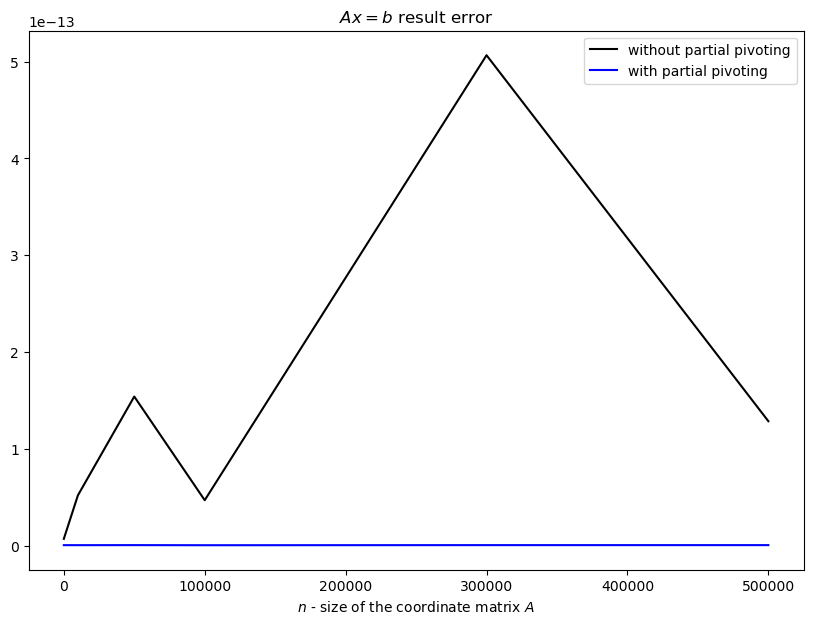
\includegraphics[width=\linewidth]{img/error.png}
        \end{subfigure}
        \hfill
        \begin{subfigure}[b]{0.45\textwidth}
            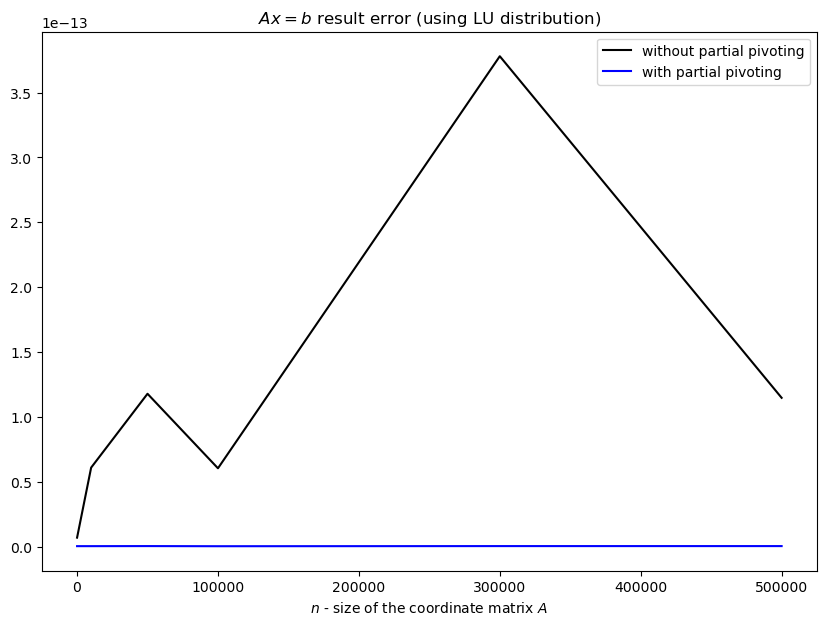
\includegraphics[width=\linewidth]{img/error_lu.png}
        \end{subfigure}
    \end{figure}

    \noindent
    Rozważmy także czas działania badanych algorytmów. Wiemy, że wyznaczenie rozkładu trójkątnego $A = LU$ macierzy wejściowej nie jest zależne od wektora prawych stron $b$. To znaczy, że dla ciągu układów równań z jedną macierzą współczynników $A$ oraz z różnymi wektorami prawych stron $b$ możemy wyznaczyć taki rozkład raz dla wszystkich wektorów $b$. W związku z tym rozwiązanie wielu układów równań z tą samą macierzą współczynników powinno być efektywniejsze dla algorytmu wykorzystującego rozkład $LU$.
    \newline\newline
    Poniższy wykres przedstawia średni czas rozwiązania jednego układu równań w ciągu układów z jedną macierzą współczynników. Na podstawie otrzymanych czasów średnich możemy potwierdzić nasze założenie.
    \newline
    Dodatkowo możemy zauważyć, że dla każdego z badanych algorytmów wyspecjalizowana implementacja struktury reprezentującej macierz $A$ o opisanej na początku strukturze okazała się mieć lepszy czas wykonywania operacji pobierania i ustawiania wartości macierzy, czego można było się spodziewać, biorąc pod uwagę fakt, że ma ona stałą złożoność czasową operacji w scenariuszu "worst case", kiedy implementacja słownikowa ma zamortyzowaną złożoność operacji $O(1)$, natomiast w scenariuszu "worst case" jest to już $O(n)$, co efektywnie pogarsza całkowitą złożoność badanych algorytmów.

    \begin{figure}[htbp]
    \centering
        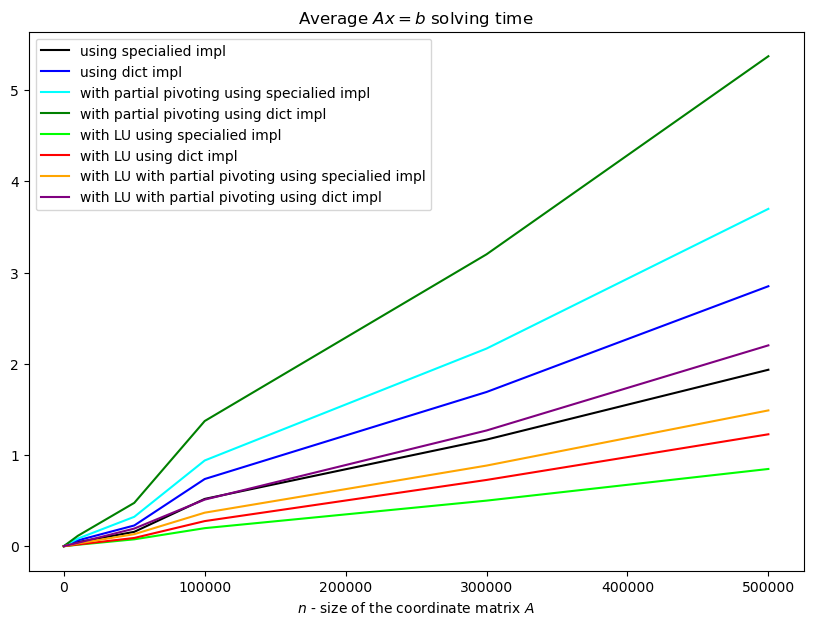
\includegraphics[width=0.68\linewidth]{img/avg_time.png}
    \end{figure}

\end{document}
